\subsection{Deployment View}
For the deployment of the project, the automated approached is chosen, which can be seen in the Deployment diagram. First of all by each merge in the master branch of the server-side of the repository the Travis CI/CD will run unit-test and integration test on the system and if all of them was successful then will check the style of the code, and if everything goes right it will make the docker image from the changed service. Then Travis CI/CD will connect to the Kubernetes through the ssh and deploys the docker image made in the previous section. Each component will be deployed in a separated container for better isolation and a further improvement of the system in the future, also each component has it owns database in a separated container for better scalability. Further, because we used the SQLAlchemy as the ORM of the system then we need a bytecode of each model (represented as an artifact) in the related REST API container, so the deployed component in the container could communicate with the associated database container.\\
To avoid a complex diagram we just showed one container Database, which is the representer of all the containers. Except for IMD container and recommender container which include the image manipulation detection and intervention recommender respectively; the reset can be scaled based on the upcoming load to more than one container but these two, because of batch execution always will be one instance of them.  Reset of the devices in the diagram is the infrastructure of other companies which provide a different kind of functionalities as service. In the reset each of the devices and their entity will be described briefly:\\
\begin{itemize}
\item \emph{Github infrastructure:} The repository of the code in one Github infrastructure which will help to have complete and distributed control one the code and also make a concrete Gitflow, to avoid conflict between different parallel feature or version of the system which are developed or are under development. Also, provide a hook for the other service like CI/CDs to access the code.\\
\item \emph{Travis-CI:} The continuous integration and delivery will use the Travis infrastructure this service will test the code in different approaches and check the style of the code. To have the same code schema and test the code to avoid crashes of the system for predictable inputs.
\item \emph{Kubernetes:} This part of the main server of the system will help to could manage container and their connection with each other to could scale them as easy as possible.
\item \emph{REST API:} each REST API container is one the subcomponent of the REST API component in the Figure (X) which the functionality of each one is described in the component view of the system. But, each of these components in the container is developed in the way that it has responsible for requests and responses related to itself, in other words, each container will handle an event end-to-end.
\item \emph{Database:} the database container is the representer of the private database for each component in the REST-API. This means each container in the REST API has its database container to have isolation between services and also could scale each part separately.
\item \emph{IMD Container:} IMD component will run a Cron job to detect the manipulated images in this component and will store the ID of the image in its database. This component, because its intrinsic property does not need scaling so always, will be one but its database could be more than one based on the speed and storage the system needed.
\item \emph{Recommender container:} This container like the IMD contain the intervention recommender which runs a job based on reports and accident to suggest some mediations for authorities.
\item \emph{DataDog:} In the monitoring of the infrastructure of the system the service of DataDog is used which allows for common monitoring tasks with simple configuration, and the Dashboard for this task is in the DataDog infrastructure and using the system just need to install a package in the host OS.
\item \emph{Sentry:} for the logging and error tracking of the system itself the service provided by the Sentry is used. The reason for this is an easy setup and configuration which sentry provides for logging and error tracking. Also, in the error tracking of the android app, this service is used again. Using this service in the system just needs to use their SDK in our system.
\item \emph{GoogleMap API:} All the functionalities related to the geo-coordination will be handled by this service because it is the most comprehensive and reasonably reliable option in the mark with proper price.
\item \emph{Firebase Infrastructure:} Firebase has different API for the developer which in the system the authentication and storage services are used. The reason behind this decision is the authentication is the reliability of this service which implementation of JWT is too much risk because of the escaped bug and it is the invention of the wheel again. In the storage part because the system needs to store the images of the violations there is a requirement for powerful multimedia storage and database. This service will solve the problem for storage without any hassle to configure and manage the storage space for this kind of file and has a fast response time.
\item \emph{Cloudflare infrastructure:} The SSL/TLS service will help the system to guarantee the security of the massages communicate between the client app and the server-side. Both the load balancing and CDN services will help to API work faster in heavy load and load the binary files faster. Firewall and rate-limiting services avoid misuse of the API by anyone who wants to use the API functionalities in abnormal numbers like bot which sends to thousands of requests in a second and also these two services will avoid DDOS attack. The DNS/DNSSEC service will map a URL to the IP of the server and also avoids the DNS attacks.
\item \emph{Android App:} unlike the rolling update of the server-side the android side has a manul deployment in which the release version of the app will be uploaded in the google play manually. The app includes two main components which one is the SQLite database for all the needs to store data on the client-side. The plate number recognition component will be upgraded by each release of the Android app.
In the final, it is necessary to describe all the communication between the service in the server that will happen by RabbitMQ and each component in the server implemented in the structure of the REST.
\end{itemize}
% \begin{sidewaysfigure}
\begin{figure}[H]
\caption{Deployment Diagram}
\label{fig:Deployment}
\centering
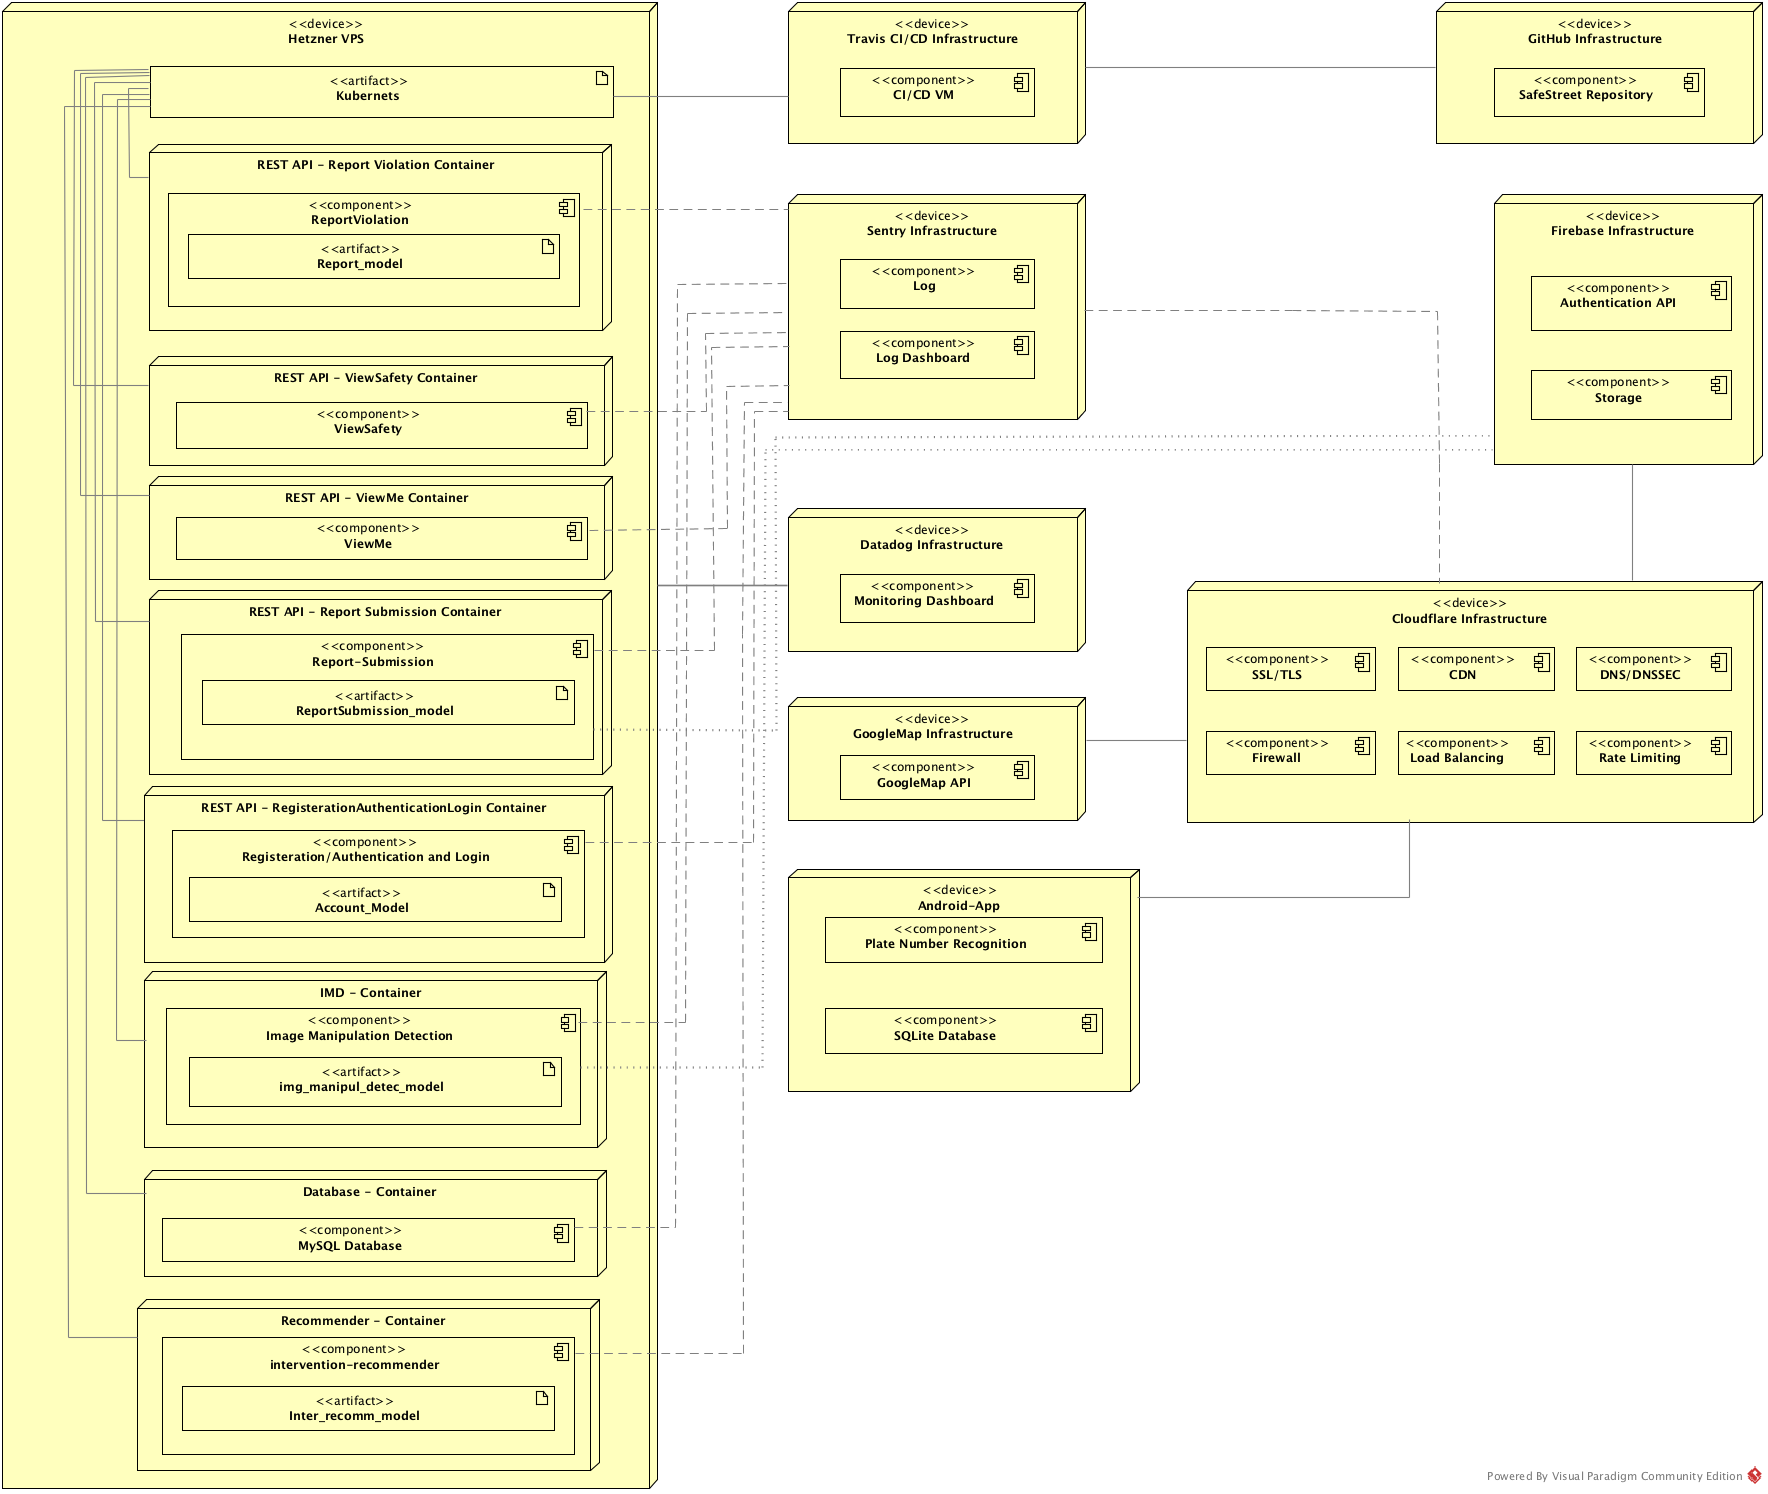
\includegraphics[width=\textwidth, height=0.8\textheight]{DeploymentDiagram.png}
\end{figure}
% \end{sidewaysfigure}
